\documentclass[10pt]{article}
\usepackage{latexsym, amssymb, graphics}
\usepackage[colorlinks=true,urlcolor=cyan]{hyperref}
\usepackage{amsmath}
\usepackage[usenames,dvipsnames]{color}
\usepackage[left=1in, right=1in, top=0.4in, bottom=0.4in]{geometry}


\usepackage{tikz}
\usetikzlibrary{arrows, decorations.markings}

\tikzstyle{vecArrow} = [thick, decoration={markings,mark=at position
   1 with {\arrow[semithick]{open triangle 60}}},
   double distance=5pt, shorten >= 5.5pt,
   preaction = {decorate},
   postaction = {draw,line width=5pt, white,shorten >= 4.5pt}]
\tikzstyle{innerWhite} = [semithick, white,line width=5pt, shorten >= 4.5pt]


\title{TLA+ Proof Manager - Specification}
\author{Jael E. Kriener}

\begin{document}

\maketitle

\section{What}

The PM interacts with its surroundings as follows:


\begin{figure}[h]

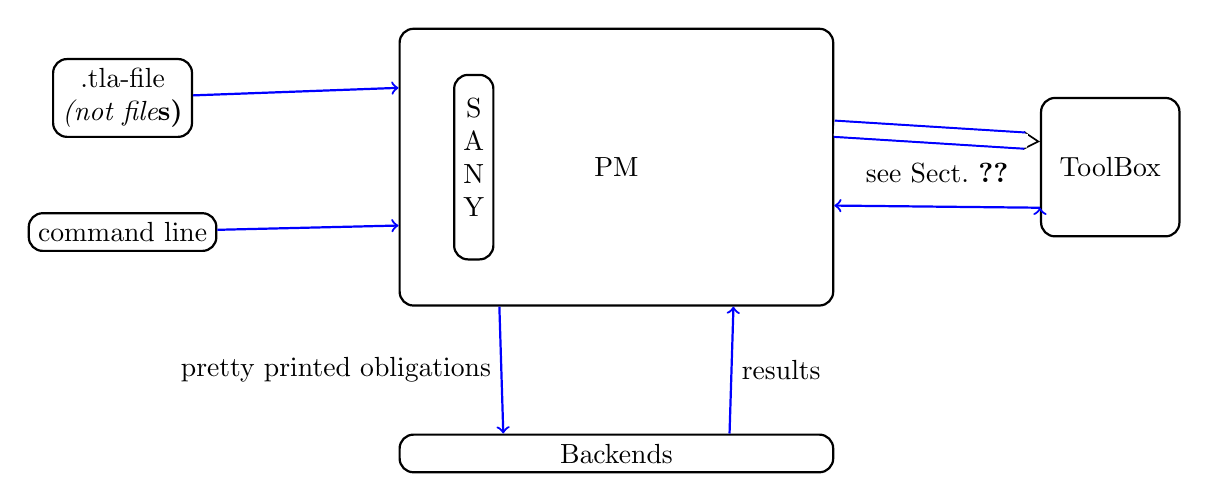
\begin{tikzpicture}[thick, main node/.style={rectangle, thick, draw, rounded corners=5, align=center}]
\node[main node] (I1) [ ] {.tla-file\\ \emph{(not file\bf{s})}}; 
\node[main node] (I2) [below of=I1, yshift=-20pt ] {command line}; 
\node[main node] (PM) [right of=I1, xshift=150pt, yshift=-25pt, text width=150, minimum size=100pt] {PM};
\node[main node] (TB) [right of=PM, xshift=150pt, minimum size=50pt] {ToolBox};
\node[main node] (BEs) [below of=PM, yshift=-75pt, text width=150pt] {Backends};
\node[main node] (SN) [right of=PM, xshift=-80pt] {\ \\S\\A\\N\\Y\\};


\path[->, rounded corners, thick, draw=blue]
(I1) edge [] node [] {} (PM.160)
(I2) edge [] node [] {} (PM.195)
(PM.230) edge [] node [left] {pretty printed obligations} (BEs.170)
(BEs.10) edge [] node [right] {results} (PM.310)
(TB.210) edge [] node [above, yshift=5pt] {see Sect.~\ref{sect:TB-PM-Comms}} (PM.350)
;

\draw[vecArrow, draw=blue] (PM.370) to (TB.160);
\end{tikzpicture}


\caption{Overview: Input-Output of the PM}
\end{figure}


\subsection{ToolBox - Proof Manager Communications Protocol}\label{sect:TB-PM-Comms}
ToDo: record 

\section{How}




\section{Code}



\end{document}
